%!TEX root = slides.tex

\section{Algorithms}

\begin{frame}{Decision tree}
  \begin{definition}
    A decision tree is a rooted tree where each vertex represents a decision. The possible results of each decision are represented by the edges connecting the vertex to the vertices at the next level down. Final outcomes of the procedure are represented by the leaves.
  \end{definition}
  \begin{center}
    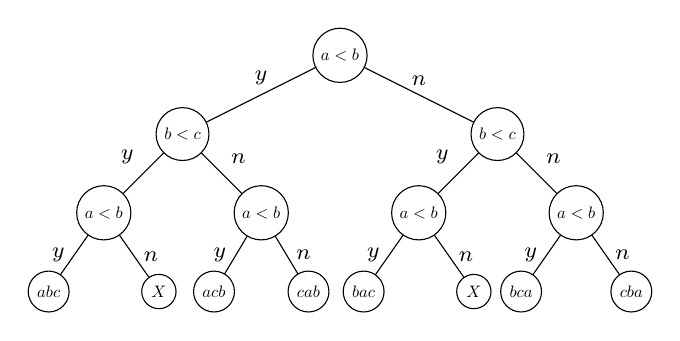
\begin{tikzpicture}
    \begin{scope}[every node/.style={circle,draw,scale=0.6}]
    \node (a) at (3,4) {$a<b$};
    \node (b) at (1,3) {$b<c$};
    \node (c) at (5,3) {$b<c$};
    \node (d) at (0,2) {$a<b$};
    \node (e) at (2,2) {$a<b$};
    \node (f) at (4,2) {$a<b$};
    \node (g) at (6,2) {$a<b$};
    \node (h) at (-0.7,1) {$abc$};
    \node (i) at (0.7,1) {$X$};
    \node (j) at (1.4,1) {$acb$};
    \node (k) at (2.6,1) {$cab$};
    \node (l) at (3.3,1) {$bac$};
    \node (m) at (4.7,1) {$X$};
    \node (n) at (5.3,1) {$bca$};
    \node (o) at (6.7,1) {$cba$};
    \end{scope}
    \begin{scope}[every edge/.style={draw=black}]
    \path (a) edge node[above] {\footnotesize $y$} (b);
    \path (a) edge node[above] {\footnotesize $n$} (c);
    \path (b) edge node[above left] {\footnotesize $y$} (d);
    \path (b) edge node[above right]  {\footnotesize $n$} (e);
    \path (c) edge node[above left] {\footnotesize $y$} (f);
    \path (c) edge node[above right]  {\footnotesize $n$} (g);
    \path (d) edge node[left] {\footnotesize $y$} (h);
    \path (d) edge node[right]  {\footnotesize $n$} (i);
    \path (e) edge node[left] {\footnotesize $y$} (j);
    \path (e) edge node[right]  {\footnotesize $n$} (k);
    \path (f) edge node[left] {\footnotesize $y$} (l);
    \path (f) edge node[right]  {\footnotesize $n$} (m);
    \path (g) edge node[left] {\footnotesize $y$} (n);
    \path (g) edge node[right]  {\footnotesize $n$} (o);
    \end{scope}
    \end{tikzpicture}
  \end{center}
\end{frame}

